%=============================================================================
% Zero-Shot Foundation Model Forecasting of Visitor Flow in Heritage Museums
% with Topology-Constrained Reconciliation
%
% Build:  pdflatex main && bibtex main && pdflatex main && pdflatex main
%
% Every number in this paper is produced by paper/Arxiv/analysis.py from the
% logged runs under results/. Nothing is transcribed by hand.
%=============================================================================

\documentclass[11pt]{article}

\usepackage{arxiv}

\usepackage[utf8]{inputenc}
\usepackage[T1]{fontenc}
\usepackage{lmodern}
\usepackage{amsmath,amssymb,amsfonts,amsthm}
\usepackage{bm}
\usepackage{booktabs}
\usepackage{graphicx}
\usepackage{subcaption}
\usepackage{xcolor}
\usepackage[numbers,sort&compress]{natbib}
\usepackage[colorlinks=true,linkcolor=black,citecolor=blue,urlcolor=blue]{hyperref}
\usepackage[protrusion=true,expansion=false]{microtype}
\usepackage{url}
\usepackage{siunitx}
\sisetup{detect-weight=true,detect-family=true}

\theoremstyle{plain}
\newtheorem{theorem}{Theorem}
\newtheorem{proposition}[theorem]{Proposition}
\newtheorem{lemma}[theorem]{Lemma}
\newtheorem{corollary}[theorem]{Corollary}
\theoremstyle{definition}
\newtheorem{definition}[theorem]{Definition}
\newtheorem{hypothesis}{Hypothesis}
\theoremstyle{remark}
\newtheorem{remark}[theorem]{Remark}

\newcommand{\bA}{\bm{A}}
\newcommand{\by}{\bm{y}}
\newcommand{\bb}{\bm{b}}
\newcommand{\bOm}{\bm{\Omega}}
\newcommand{\yhat}{\hat{\by}}
\newcommand{\ytil}{\tilde{\by}}
\newcommand{\cY}{\mathcal{Y}}
\newcommand{\Rb}{\mathbb{R}}
\newcommand{\best}[1]{\textbf{#1}}

% Float placement. The results section queues seven floats in quick succession,
% and the stock parameters are too tight to place them, which deadlocks the
% float queue rather than merely producing ugly pages.
\setcounter{topnumber}{3}
\setcounter{bottomnumber}{2}
\setcounter{totalnumber}{5}
\renewcommand{\topfraction}{0.9}
\renewcommand{\bottomfraction}{0.7}
\renewcommand{\textfraction}{0.07}
\renewcommand{\floatpagefraction}{0.7}

\settitlerunning{Zero-Shot Forecasting of Museum Visitor Flow}
\renewcommand{\headeright}{Preprint}

\title{Zero-Shot Foundation Model Forecasting of Visitor Flow\\in Heritage Museums with Topology-Constrained Reconciliation}

\author{
  A. A. Jafari, C. Ozcinar\\
  University of Tartu \\
  Tartu, Estonia \\
  \texttt{\{akbar.anbar.jafari\}@ut.ee} \\
  %% examples of more authors
   \And
  G. Anbarjafari \\
  3S Holding OÜ \\
  Tartu, Estonia\\
  \texttt{shb@3sholding.com} \\
}

\date{\today}

\begin{document}
\maketitle

\begin{abstract}
European museums are overwhelmingly housed in protected heritage buildings, where structural intervention is restricted and dense visitor flow threatens people, fabric and collection at once. Data-driven crowd management is blocked by a practical obstacle: predictive models need historical data from the specific building, and almost no heritage museum has any. We ask whether a pre-trained time series foundation model can close that gap, and we find that the answer depends, in a way that is both measurable and predictable in advance, on a single property of the signal. We formulate indoor visitor dynamics as multivariate forecasting on a building graph, with room occupancy as node series and directional doorway counts as edge series. Because such models are topology-blind, we introduce an uncertainty-weighted constrained projection that maps a raw forecast onto the physically admissible set defined by discrete mass conservation, non-negativity and room capacity, using the model's own quantile spread as the metric. We prove the projection is unique, exactly coherent, and non-expansive towards any admissible truth, and we show that classical minimum trace reconciliation is the special case that drops the inequality constraints. Empirically, across \num{783} forecast origins of real room occupancy, \num{543} to \num{588} origins of real metro flow and \num{300} origins of a simulated museum, three foundation models are compared against five baselines. We state and test the hypothesis that the zero-shot advantage is a decreasing function of the daily seasonal strength $S_m$ of the target. It holds without exception: at $S_m=0.44$ the best zero-shot model beats every local baseline by \SI{14.9}{\percent} MASE at one hour and the margin is significant under a Diebold-Mariano test, at $S_m=0.55$ the advantage is $-\SI{4.0}{\percent}$, and at $S_m=0.79$ it is $-\SI{33.5}{\percent}$ and no foundation model significantly beats a seasonal baseline at any horizon. The reverse holds for uncertainty: the baselines that win on point accuracy emit intervals covering \SI{4}{\percent} of outcomes against a nominal \SI{80}{\percent}, whereas the foundation models reach \SI{75}{\percent} to \SI{91}{\percent}. Raw forecasts violate conservation by \num{1.05} persons per node per interval; the proposed projection removes this exactly, introduces no bound violation, reduces MAE by \SI{0.76}{\percent} $(p=\num{1.2e-2})$ and beats uniform weighting by \SI{1.03}{\percent} $(p=\num{8.5e-34})$ in \SI{10.2}{\milli\second}. We release the benchmark, the reconciliation layer and the evaluation harness.
\end{abstract}

\noindent\textbf{Keywords:} time series foundation models \textendash{} zero-shot forecasting \textendash{} hierarchical reconciliation \textendash{} crowd flow \textendash{} cultural heritage \textendash{} occupancy prediction

%=============================================================================
\section{Introduction}
%=============================================================================

A museum in a protected building cannot be widened. Doorways, staircases and egress capacity are fixed by law as much as by masonry, and the only variable left to an operator is when and where visitors are asked to go. Three distinct risks converge on the same physical quantity, namely how many people are in which space and where they are heading next. Crowd safety depends on density at bottlenecks. Conservation of fabric and collection depends on cumulative visitor-induced heat, moisture and carbon dioxide rather than on instantaneous peaks \citep{camuffo2019,en15757}. Security depends on movement that does not match the pattern of the day. All three are served by one forecast and differ only in the decision rule applied on top of it.

The obstacle is not modelling but data. The mature literature on spatio-temporal flow forecasting was developed for road traffic and metro ridership, where months of history from the network being forecast are available as a matter of course. Graph neural models such as DCRNN \citep{li2018dcrnn}, STGCN \citep{yu2018stgcn} and Graph WaveNet \citep{wu2019graphwavenet} are trained per network and are not defined on an unseen topology. Heritage museums are precisely where that assumption fails: they are small, numerous, individually under-resourced, and mostly uninstrumented, and a newly instrumented site yields no usable training data for weeks. A method that needs a year of data before its first useful forecast will not be deployed in this sector.

Time series foundation models offer a way out of the cold start, since they forecast unseen series with no task-specific training \citep{das2024timesfm,ansari2024chronos,woo2024moirai}. The current generation is natively multivariate, fills the whole horizon in one forward pass, and accepts covariates whose future values are known at forecast time \citep{timesfm3,ansari2025chronos2,khwaja2026toto2}, which matches museum operations closely, since timed entry slots and tour departures are known in advance. Two questions have not been answered. Whether pre-training transfers to indoor room-level human flow at all is open, because the standard benchmarks are dominated by retail, energy, finance and observability data \citep{aksu2024gifteval} and indoor occupancy is bounded above by capacity, bursty, frequently zero, and driven by scheduled events. And whether a topology-blind forecaster can be made to respect the building is open, because nothing in these architectures encodes that the quantities they emit are coupled by conservation of mass.

This paper answers both, and in doing so replaces a question that turns out to be badly posed. Asking whether zero-shot forecasting beats local baselines admits no general answer, because we find the sign of the effect reverses across settings that look superficially similar. We therefore state and test a sharper claim: the zero-shot advantage is governed by how much of the target's variance a periodic profile already explains. Where that fraction is low the foundation models win decisively, and where it is high a seasonal baseline that costs \SI{3}{\milli\second} is not displaced at all. Stating the claim this way makes it falsifiable, makes it actionable before any model is run, and, as Section~\ref{sec:results} shows, makes it correct on every dataset we tested.

\paragraph{Contributions.}
\begin{enumerate}\itemsep2pt
\item A formulation of indoor visitor flow forecasting as multivariate forecasting on a building graph, with node occupancy, signed edge flow and operational covariates, designed so that a general purpose forecaster applies without modification (Section~\ref{sec:formulation}).
\item An uncertainty-weighted topology-constrained projection that makes any quantile forecaster physically admissible, with proofs of uniqueness, exact coherence and non-expansiveness towards an admissible truth, and a proposition placing MinT as the special case that discards the inequality constraints (Section~\ref{sec:method}).
\item A falsifiable predictability hypothesis for when zero-shot forecasting helps, stated in a statistic computable from the target history alone and before any forecast is made, and confirmed on three datasets spanning $S_m \in [0.44, 0.79]$ (Sections~\ref{sec:hypotheses} and~\ref{sec:results}).
\item The first evaluation of time series foundation models on indoor room-level occupancy, over \num{783} rolling origins with paired Diebold-Mariano testing under Holm correction, together with a measurement of how badly such models violate building topology and of what it costs to repair it (Section~\ref{sec:results}).
\item An open simulated heritage museum benchmark with full ground truth on every doorway, plus the reconciliation layer and a harness in which every artefact is traceable to a logged run.
\end{enumerate}

%=============================================================================
\section{Related work}
\label{sec:related}
%=============================================================================

The problem sits where four literatures meet, which have so far developed largely independently.

\paragraph{From describing visitors to predicting them.}
Museum circulation study began with observational ethnography. \citet{veron1983} proposed the typology of visiting styles that still organises the field, distinguishing the \emph{ant}, who follows the suggested route and stops often, the \emph{fish}, who traverses open space with few stops, the \emph{butterfly}, who changes direction and revisits, and the \emph{grasshopper}, who targets a few exhibits. Later work quantified the regularities that emerge when many such visitors share a building, documenting turning biases, an attraction towards exits growing with elapsed time, and declining stopping behaviour \citep{klein1993,bitgood2006}, and connected them to the morphology of the layout itself \citep{choi1999}. Pervasive sensing changed the resolution but not the orientation \citep{kanda2007,yoshimura2014louvre,uwbmuseum2026}. Modelling gallery transitions as a random walk \citep{yoshimura2019randomwalk} gives the simplest predictive model, $\pi_{t+1}^{\top} = \pi_t^{\top}\bm{P}$, which we treat as a baseline in spirit: it is homogeneous in time, blind to scheduled events and incapable of expressing uncertainty. The closest prior work \citep{centorrino2021museums} measures and optimises a known configuration, whereas our objective is to predict a specific quantity a fixed interval ahead with calibrated uncertainty, so that an intervention can be made before the state is reached.

\paragraph{Observing occupancy without altering the building.}
Conservation monitoring already instruments heritage buildings for unrelated reasons, and those signals are informative about occupancy. For a well-mixed zone of volume $V$, ventilation rate $Q$, outdoor concentration $C_{\mathrm{out}}$, per-person generation $G$ and occupancy $n(t)$,
\begin{equation}
V\frac{\mathrm{d}C(t)}{\mathrm{d}t} = G\,n(t) - Q\left(C(t) - C_{\mathrm{out}}\right),
\label{eq:co2}
\end{equation}
so a step in occupancy is followed exponentially with time constant $\tau = V/Q$. Equation~\eqref{eq:co2} explains both why carbon dioxide is useful and why it is insufficient alone, since $\tau$ of tens of minutes means the signal reports the recent past. \citet{candanedo2016} demonstrated occupancy detection from light, temperature, humidity and carbon dioxide, and \citet{chen2018review} survey the field. ROBOD \citep{tekler2022robod} and the dataset of \citet{schwee2019} provide room-level ground truth counts alongside such signals, and we use the former precisely because it lets the lag be measured rather than assumed. Direct doorway counting is more immediate but errs most in dense and grouped flow \citep{brscic2013}. Every available observation is therefore a lagged, noisy and partially missing view of a latent state.

\paragraph{Flow on networks.}
The machine learning literature on forecasting flow over physical networks is mature. \citet{li2018dcrnn} model spatial dependence as diffusion on the graph, \citet{yu2018stgcn} combine graph and temporal convolution, \citet{wu2019graphwavenet} learn an adaptive adjacency, and attention variants followed \citep{guo2019astgcn,zheng2020gman}. Closest to our setting, \citet{liu2022pvcgn} forecast station-level metro inflow and outflow on a physical network, which we adopt both as a baseline family and as real evaluation data, since a metro network satisfies the same continuity equation a museum does. Two cautions follow. \citet{shao2022stid} showed much of the reported advantage of graph models comes from learned identity embeddings rather than topology, so any claim that topology helps needs a careful ablation. And every model in this family is trained on the network it forecasts, which is the requirement heritage museums cannot meet.

\paragraph{Foundation models.}
\citet{das2024timesfm} introduced a decoder-only transformer that partitions a series into patches, embeds each as a token and predicts future patches. Related designs differ mainly in tokenisation and uncertainty representation \citep{ansari2024chronos,woo2024moirai,goswami2024moment}, and compact variants show that competitive zero-shot accuracy does not require large parameter counts \citep{ekambaram2024ttm}, which matters for on-premise inference. The current generation decodes the whole horizon in one pass following the masking scheme of \citet{auer2025tirex}, alternates causal attention along time with full attention across variates \citep{khwaja2026toto2,timesfm3}, and accepts known-future covariates \citep{timesfm3,ansari2025chronos2}. Uncertainty comes from a quantile head trained with the pinball loss, $\mathcal{L}_{\alpha}(y,\hat{y}^{(\alpha)}) = \max\{\alpha(y-\hat{y}^{(\alpha)}),\,(\alpha-1)(y-\hat{y}^{(\alpha)})\}$, which in this work supplies not only the reported intervals but the metric of the projection in Section~\ref{sec:method}.

\paragraph{Coherence.}
Hierarchical forecasting has addressed a structurally similar problem for two decades. With $\by = \bm{S}\bm{b}$ and base forecasts that violate it, reconciliation applies a linear map $\ytil = \bm{S}\bm{P}\yhat$; \citet{hyndman2011optimal} proposed the least squares choice and \citet{wickramasuriya2019mint} derived the minimum trace solution $\bm{P} = (\bm{S}^{\top}\bm{W}^{-1}\bm{S})^{-1}\bm{S}^{\top}\bm{W}^{-1}$, showing reconciliation reduces expected squared error. \citet{panagiotelis2021geometric} recast it as projection onto the coherent subspace, the view we adopt and generalise. Extensions address non-negativity \citep{wickramasuriya2020nonneg}, regularisation \citep{bentaieb2019regularized} and end-to-end coherent probabilistic forecasting \citep{rangapuram2021endtoend}. Two differences prevent direct reuse here, and Section~\ref{sec:method} makes them precise: our constraint is not an aggregation hierarchy but a general linear coupling across time and incident edges, and our admissible set is bounded, so the correction is a constrained projection rather than a linear map. Critically, MinT requires an estimated error covariance, which presupposes a forecast error history at the site and so reintroduces the cold start we set out to avoid.

\paragraph{Decisions, simulation and privacy.}
The level of service framework \citep{fruin1971} expresses circulation quality as area per person, and crowd disasters show the transition to danger is abrupt and preceded by measurable changes in the flow field \citep{helbing2007crowd}. Departure from a predictive interval is a natural alarm statistic whose false alarm rate can be controlled distribution-free by conformal methods for sequential data \citep{stankeviciute2021conformal,xu2021enbpi} and under shift \citep{gibbs2021adaptive}; the wider area is surveyed by \citet{blazquez2021review}. Evaluating conservation violation requires knowing true flow on every doorway simultaneously, which no real deployment provides, so pedestrian simulation is the standard substitute \citep{helbing1995social,seitz2012osm,kleinmeier2019vadere,jupedsim}. Finally, systematic monitoring in publicly accessible areas attracts a data protection impact assessment under Article 35 of the GDPR \citep{gdpr}. Our formulation is deliberately aggregate: the forecast state is a vector of counts, no trajectory is retained and no identifier is formed. That is a methodological constraint, not a disclaimer, since it is exactly why the problem is posed as forecasting on a graph rather than as trajectory prediction.

\paragraph{The gap.}
Museum studies describe movement richly but retrospectively. Spatio-temporal models could predict it but presuppose a history heritage museums lack, while the foundation models that remove that requirement have not been evaluated on indoor room-level flow at all. And no forecaster in either family is aware of conservation, so its outputs are not physically admissible, while the reconciliation machinery that could impose admissibility was built for aggregation hierarchies with estimated error covariances rather than for bounded flow networks under zero-shot conditions. This paper addresses the three together.

%=============================================================================
\section{Problem formulation}
\label{sec:formulation}
%=============================================================================

\subsection{The building as a graph}

Represent the museum as a directed graph $G=(V,E)$ whose nodes are galleries, halls, stairwells and entrances, and whose edges are doorways, one edge per direction. We close the graph with a single virtual node $v_{\mathrm{out}} \in V$ representing the exterior, so that every visitor who enters or leaves the building crosses an edge incident to it. Write $V_{\mathrm{int}} = V \setminus \{v_{\mathrm{out}}\}$ for the interior.

For node $v$ and discrete time $t$ let $o_v(t) \in \Rb_{\ge 0}$ be the occupancy at the end of interval $t$, and for directed edge $e$ let $f_e(t) \in \Rb_{\ge 0}$ be the number of crossings during interval $t$. Because the graph is closed and visitors are neither created nor destroyed, for every interior node
\begin{equation}
o_v(t) - o_v(t-1) - \sum_{e \in \mathrm{in}(v)} f_e(t) + \sum_{e \in \mathrm{out}(v)} f_e(t) \;=\; 0,
\qquad \forall v \in V_{\mathrm{int}}.
\label{eq:conservation}
\end{equation}
Equation~\eqref{eq:conservation} is the discrete continuity equation and is the single structural fact separating this problem from a generic collection of correlated series. It is exact by construction, not an approximation: it holds for the true counts whenever the sampling interval is short enough that no visitor traverses two doorways within one step, a condition satisfied at the one to five minute resolutions used here.

\subsection{Forecast target and the admissible set}

Fix a forecast origin $t_0$ and a horizon $H$. The forecaster emits, for each target series and each step $h \in \{1,\dots,H\}$, the quantiles $\{\hat{y}^{(\alpha)}\}$ at levels $\alpha \in \mathcal{A} = \{0.1,\dots,0.9\}$. Stack the median forecasts for all $n = |V_{\mathrm{int}}| + |E|$ series and all $H$ steps into a single vector $\yhat \in \Rb^{m}$, $m = nH$, ordering occupancy series before flow series.

Applying~\eqref{eq:conservation} at every interior node and every step gives $|V_{\mathrm{int}}|\cdot H$ linear equations in $\by$. Collecting them,
\begin{equation}
\bA \by = \bb,
\qquad
\bA \in \Rb^{k \times m},\quad k = |V_{\mathrm{int}}| \cdot H,
\label{eq:system}
\end{equation}
where $\bA$ carries the node-edge incidence structure and the coupling between consecutive steps, and $\bb$ is zero except in the rows for $h=1$, which absorb the last observed occupancies $o_v(t_0)$. The anchor is the only place observed data enters the constraint, and it is observed strictly before the origin, so the constraint leaks nothing about the evaluation window.

Counts are non-negative and rooms have finite capacity $c_v$, so the admissible set is
\begin{equation}
\cY \;=\; \left\{ \by \in \Rb^m \;:\; \bA\by = \bb, \;\; \bm{l} \le \by \le \bm{u} \right\},
\qquad
l_i = 0, \quad
u_i = \begin{cases} c_{v(i)} & \text{$i$ an occupancy coordinate},\\ +\infty & \text{$i$ a flow coordinate}.\end{cases}
\label{eq:admissible}
\end{equation}

\begin{proposition}[Structure of $\cY$]
\label{prop:convex}
$\cY$ is a closed convex set. It is non-empty whenever the anchor is itself admissible, that is $0 \le o_v(t_0) \le c_v$ for all $v \in V_{\mathrm{int}}$.
\end{proposition}
\begin{proof}
$\cY$ is an intersection of the affine set $\{\bA\by = \bb\}$ with the box $[\bm{l},\bm{u}]$, both closed and convex, so $\cY$ is closed and convex. For non-emptiness, take $\by^{0}$ with all flow coordinates zero and all occupancy coordinates equal to the anchor, $o_v(t_0+h) = o_v(t_0)$ for every $h$. Every balance in~\eqref{eq:conservation} then reads $o_v(t_0)-o_v(t_0)-0+0=0$, which holds, and $\by^{0}$ lies in the box by the assumption on the anchor. Hence $\by^{0} \in \cY$.
\end{proof}

Proposition~\ref{prop:convex} matters operationally: the "nobody moves" forecast is always admissible, so the projection of Section~\ref{sec:method} can never be infeasible for a building whose observed occupancy is within capacity. We therefore never need a fallback that silently relaxes physics.

%=============================================================================
\section{Topology-constrained reconciliation}
\label{sec:method}
%=============================================================================

\subsection{The projection}

A foundation model has no representation of the floor plan, so $\yhat \notin \cY$ in general. We repair it by moving as little as possible, in a metric supplied by the model's own uncertainty:
\begin{equation}
\ytil \;=\; \arg\min_{\by \in \cY} \; (\by - \yhat)^{\top} \bOm \, (\by - \yhat),
\qquad
\bOm = \mathrm{diag}\!\left(\sigma_1^{-2},\dots,\sigma_m^{-2}\right),
\label{eq:qp}
\end{equation}
where $\sigma_i$ is read off the predicted interval. Taking the nominal \SI{80}{\percent} band to be Gaussian in width,
\begin{equation}
\sigma_i \;=\; \frac{\hat{y}^{(0.9)}_i - \hat{y}^{(0.1)}_i}{2 z_{0.9}},
\qquad z_{0.9} \approx 1.2816,
\qquad \text{so} \quad 2 z_{0.9} \approx 2.5631 .
\label{eq:sigma}
\end{equation}
The design intent is that series the model is confident about are moved little, and series it is unsure about absorb the correction. The foundation model supplies both the forecast and the information about where the forecast can safely be bent; the building supplies the constraints. In practice $\sigma_i$ is floored at a small $\varepsilon>0$ so that $\bOm$ is finite, which is needed because a model may emit a degenerate interval on a series that is identically zero.

\begin{theorem}[Existence, uniqueness and coherence]
\label{thm:unique}
Let $\cY \ne \emptyset$ and let $\sigma_i \ge \varepsilon > 0$ for all $i$. Then problem~\eqref{eq:qp} has a unique solution $\ytil$, and it satisfies $\bA\ytil = \bb$ and $\bm{l}\le\ytil\le\bm{u}$ exactly.
\end{theorem}
\begin{proof}
Since $\sigma_i \ge \varepsilon$, we have $\bOm \succeq \varepsilon^{-2}\bm{I} \succ 0$, so the objective $\phi(\by) = (\by-\yhat)^{\top}\bOm(\by-\yhat)$ is strongly convex with modulus $2\varepsilon^{-2}$ and is coercive. By Proposition~\ref{prop:convex}, $\cY$ is non-empty, closed and convex. A coercive continuous function attains its infimum on a non-empty closed set, giving existence. For uniqueness, suppose $\by_1 \ne \by_2$ both attain the minimum $\phi^\star$. By convexity of $\cY$ their midpoint lies in $\cY$, and strong convexity gives
$\phi\!\left(\tfrac{\by_1+\by_2}{2}\right) \le \tfrac{1}{2}\phi(\by_1) + \tfrac{1}{2}\phi(\by_2) - \tfrac{1}{4}\cdot 2\varepsilon^{-2}\|\by_1-\by_2\|_2^2 < \phi^\star$,
contradicting minimality. Coherence and feasibility hold because $\ytil \in \cY$ by construction, and membership of $\cY$ is exactly the conjunction of $\bA\ytil=\bb$ and the box constraints.
\end{proof}

Theorem~\ref{thm:unique} is what distinguishes a constraint from a penalty. A soft conservation loss added to a training objective yields forecasts that are approximately coherent by an amount nobody controls. Here the residual is zero up to solver tolerance, which we verify empirically in Section~\ref{sec:results} at $\num{4e-9}$ persons.

\subsection{Why the projection cannot hurt, and in what sense}

Write $\|\bm{z}\|_{\bOm}^2 = \bm{z}^{\top}\bOm\bm{z}$ and let $\Pi_{\cY}$ denote the map $\yhat \mapsto \ytil$ of~\eqref{eq:qp}, the projection onto $\cY$ in the $\bOm$-metric.

\begin{lemma}[Variational inequality]
\label{lem:vi}
$\ytil = \Pi_{\cY}(\yhat)$ if and only if $\ytil \in \cY$ and
$(\yhat - \ytil)^{\top}\bOm\,(\by - \ytil) \le 0$ for all $\by \in \cY$.
\end{lemma}
\begin{proof}
For $\by \in \cY$ and $\lambda \in (0,1]$, convexity gives $\ytil + \lambda(\by-\ytil) \in \cY$. Optimality of $\ytil$ gives $\phi(\ytil + \lambda(\by-\ytil)) \ge \phi(\ytil)$. Expanding,
\[
\phi(\ytil+\lambda(\by-\ytil)) - \phi(\ytil)
= 2\lambda\,(\ytil-\yhat)^{\top}\bOm(\by-\ytil) + \lambda^{2}\|\by-\ytil\|_{\bOm}^{2} \;\ge\; 0 .
\]
Dividing by $\lambda>0$ and letting $\lambda \downarrow 0$ yields $(\ytil-\yhat)^{\top}\bOm(\by-\ytil) \ge 0$, which is the stated inequality. Conversely, if the inequality holds then for any $\by \in \cY$,
$\phi(\by) - \phi(\ytil) = 2(\ytil-\yhat)^{\top}\bOm(\by-\ytil) + \|\by-\ytil\|_{\bOm}^{2} \ge \|\by-\ytil\|_{\bOm}^{2} \ge 0$,
so $\ytil$ is optimal.
\end{proof}

\begin{theorem}[The projection never moves away from an admissible truth]
\label{thm:contraction}
Let $\by^{\star} \in \cY$ be the true future. Then
\begin{equation}
\left\| \ytil - \by^{\star} \right\|_{\bOm}^{2}
\;\le\;
\left\| \yhat - \by^{\star} \right\|_{\bOm}^{2}
\;-\;
\left\| \yhat - \ytil \right\|_{\bOm}^{2}
\;\le\;
\left\| \yhat - \by^{\star} \right\|_{\bOm}^{2}.
\label{eq:contraction}
\end{equation}
The improvement is strict whenever $\yhat \notin \cY$.
\end{theorem}
\begin{proof}
Decompose $\ytil - \by^{\star} = (\yhat - \by^{\star}) - (\yhat - \ytil)$ and expand in the $\bOm$-inner product:
\[
\|\ytil-\by^{\star}\|_{\bOm}^{2}
= \|\yhat-\by^{\star}\|_{\bOm}^{2} - 2(\yhat-\ytil)^{\top}\bOm(\yhat-\by^{\star}) + \|\yhat-\ytil\|_{\bOm}^{2}.
\]
Write $(\yhat-\by^{\star}) = (\yhat-\ytil) + (\ytil-\by^{\star})$ in the cross term, giving
$(\yhat-\ytil)^{\top}\bOm(\yhat-\by^{\star}) = \|\yhat-\ytil\|_{\bOm}^{2} + (\yhat-\ytil)^{\top}\bOm(\ytil-\by^{\star})$.
By Lemma~\ref{lem:vi} with $\by = \by^{\star} \in \cY$, the last term is non-negative, since Lemma~\ref{lem:vi} states $(\yhat-\ytil)^{\top}\bOm(\by^{\star}-\ytil) \le 0$. Substituting,
\[
\|\ytil-\by^{\star}\|_{\bOm}^{2}
\le \|\yhat-\by^{\star}\|_{\bOm}^{2} - 2\|\yhat-\ytil\|_{\bOm}^{2} + \|\yhat-\ytil\|_{\bOm}^{2}
= \|\yhat-\by^{\star}\|_{\bOm}^{2} - \|\yhat-\ytil\|_{\bOm}^{2},
\]
which is~\eqref{eq:contraction}. If $\yhat \notin \cY$ then $\ytil \ne \yhat$ and $\|\yhat-\ytil\|_{\bOm}^{2}>0$, so the inequality is strict.
\end{proof}

\begin{corollary}[Expected error reduction]
\label{cor:expected}
If the true future is admissible almost surely, then $\mathbb{E}\|\ytil-\by^{\star}\|_{\bOm}^{2} \le \mathbb{E}\|\yhat-\by^{\star}\|_{\bOm}^{2}$, with the gap equal to $\mathbb{E}\|\yhat-\ytil\|_{\bOm}^{2}$, the mean squared physical implausibility of the raw forecast.
\end{corollary}

Corollary~\ref{cor:expected} is the MinT theorem of \citet{wickramasuriya2019mint} generalised from an aggregation subspace to an arbitrary closed convex admissible set, and it is worth being precise about what it does and does not promise. It is stated in the $\bOm$-weighted squared norm. Our reported accuracy metric is mean absolute error, which is a different functional, so Theorem~\ref{thm:contraction} does \emph{not} imply that MAE must improve. This is not a technicality but the crux of the empirical question, and it is why Section~\ref{sec:results} compares weighting schemes rather than assuming the guarantee transfers. What the theory does deliver is a clean explanation of the mechanism: the guaranteed gain is measured in $\bOm$, so a choice of $\bOm$ that reflects where the forecast is genuinely weak converts the guarantee into a gain that survives in other metrics, whereas $\bOm = \bm{I}$ spends the correction indiscriminately. Hypothesis~\ref{hyp:weights} makes this testable and Table~\ref{tab:recon} tests it.

\subsection{Relation to minimum trace reconciliation}

\begin{proposition}[MinT is the unbounded special case]
\label{prop:mint}
Suppose the box in~\eqref{eq:admissible} is dropped, so $\cY_{\mathrm{eq}} = \{\by : \bA\by=\bb\}$, and let $\bOm = \bm{W}^{-1}$ for a positive definite $\bm{W}$. Then~\eqref{eq:qp} has the closed form
\begin{equation}
\ytil = \yhat - \bm{W}\bA^{\top}\left(\bA\bm{W}\bA^{\top}\right)^{+}\left(\bA\yhat - \bb\right),
\label{eq:mintform}
\end{equation}
which is a linear map of $\yhat$ and coincides with minimum trace reconciliation when $\bA$ encodes an aggregation hierarchy and $\bm{W}$ is the base forecast error covariance. In general $\ytil$ of~\eqref{eq:mintform} need not satisfy $\bm{l}\le\ytil\le\bm{u}$.
\end{proposition}
\begin{proof}
With equality constraints only, the Lagrangian is $\phi(\by) + 2\bm{\lambda}^{\top}(\bA\by-\bb)$ and stationarity gives $\bOm(\by-\yhat) + \bA^{\top}\bm{\lambda} = \bm{0}$, so $\by = \yhat - \bm{W}\bA^{\top}\bm{\lambda}$. Imposing $\bA\by=\bb$ gives $\bA\bm{W}\bA^{\top}\bm{\lambda} = \bA\yhat - \bb$, and substituting the minimum-norm solution $\bm{\lambda} = (\bA\bm{W}\bA^{\top})^{+}(\bA\yhat-\bb)$ yields~\eqref{eq:mintform}. Linearity is immediate. For the final claim it suffices to exhibit one instance: a single room with capacity $c$, anchor $o(t_0)=0$, and a raw forecast assigning a large positive inflow and zero occupancy. The correction distributes the imbalance along the occupancy coordinate without reference to $c$, and for a sufficiently large forecast inflow the reconciled occupancy exceeds $c$.
\end{proof}

Proposition~\ref{prop:mint} predicts a specific empirical failure. MinT will achieve coherence, because it enforces $\bA\by=\bb$ exactly, while producing forecasts that are physically impossible in a second sense, namely negative counts or occupancies above capacity. Section~\ref{sec:results} observes exactly this, at \num{1.74} persons of bound violation per origin. It also makes the cold start argument concrete: MinT needs $\bm{W}$, an error covariance that can only be estimated from a history of forecast errors at the site, whereas~\eqref{eq:sigma} reads the metric off a single forward pass and so keeps the pipeline genuinely zero-shot.

\subsection{Quantile reconciliation and cost}

The projection acts on the median. To keep the whole predictive distribution coherent we apply the \emph{shift} strategy, translating every quantile level of series $i$ and step $h$ by the correction applied to its median, $\tilde{y}^{(\alpha)}_{ih} = \hat{y}^{(\alpha)}_{ih} + (\tilde{y}^{(0.5)}_{ih} - \hat{y}^{(0.5)}_{ih})$. This preserves the interval widths and, because it is a common translation, preserves quantile ordering, so no crossing is introduced. It is the conservative choice: it changes location without asserting that the projection has taught us anything about spread.

Problem~\eqref{eq:qp} is a convex quadratic program with $m = nH$ variables and $k = |V_{\mathrm{int}}|H$ equalities. We solve it with OSQP \citep{osqp} through a DPP-compliant parameterised CVXPY \citep{cvxpy} problem that is built once and reused across origins, so the sparsity pattern is factorised a single time. Section~\ref{sec:results} measures a median of \SI{10.2}{\milli\second} per origin at $m=\num{1440}$, which is negligible beside the \SIrange{75}{676}{\milli\second} of the forecast itself.

%=============================================================================
\section{Hypotheses}
\label{sec:hypotheses}
%=============================================================================

We state each hypothesis so that it can be falsified by the experiments of Section~\ref{sec:results}, and we name the falsifying observation explicitly. The first three concern when zero-shot forecasting is the right tool, and the last two concern the reconciliation layer.

The organising quantity is the extent to which a target is already explained by a periodic profile, since that is precisely what the cheapest competing method exploits.

\begin{definition}[Daily seasonal strength]
\label{def:strength}
For a series $y_t$ observed at interval $\Delta$ with daily period $m = \lceil 86400/\Delta \rceil$, let $\bar{y}^{(m)}_{p}$ be the mean of all observations whose index satisfies $t \equiv p \pmod m$. The daily seasonal strength is
\begin{equation}
S_m \;=\; 1 \;-\; \frac{\operatorname{Var}\!\left(y_t - \bar{y}^{(m)}_{t \bmod m}\right)}{\operatorname{Var}(y_t)} \;\in\; (-\infty, 1].
\label{eq:strength}
\end{equation}
\end{definition}
$S_m$ is zero when the time of day carries no information and approaches one when the series is a deterministic function of phase. It is computed from the training window alone, needs no forecast, and is available before any model is chosen, which is what makes a hypothesis stated in it useful rather than merely descriptive.

\begin{hypothesis}[Zero-shot transfer to indoor occupancy]
\label{hyp:transfer}
A pre-trained foundation model, given no site-specific training, forecasts real room-level occupancy better than every trivial baseline at horizons of \SIrange{30}{60}{\minute}, and the margin is statistically significant under a Diebold-Mariano test with multiplicity control.
\emph{Falsified if} no foundation model attains a significant improvement over the best baseline at either horizon.
\end{hypothesis}

\begin{hypothesis}[The predictability boundary]
\label{hyp:boundary}
The zero-shot advantage over the best local baseline is a decreasing function of the daily seasonal strength of the target, and changes sign at intermediate $S_m$. Where $S_m$ is high, a seasonal baseline is not displaced on point accuracy.
\emph{Falsified if} the ordering of the advantage across datasets does not follow the ordering of $S_m$, or if a foundation model significantly beats the seasonal baseline on the highest-$S_m$ dataset.
\end{hypothesis}

Hypothesis~\ref{hyp:boundary} is the central claim of the paper, and it is deliberately risky. It predicts the sign of an effect on an unseen dataset from a statistic of that dataset's history, and a single dataset with high $S_m$ on which a foundation model wins point accuracy refutes it.

\begin{hypothesis}[Point accuracy and uncertainty come apart]
\label{hyp:uncertainty}
Where a periodic baseline wins on point accuracy, it does not follow that it should be deployed, because the same baselines are severely miscalibrated. Foundation models attain empirical coverage close to nominal, and lower CRPS at short horizons, even on datasets where they lose on MASE.
\emph{Falsified if} the baselines that win on MASE also attain coverage within a few points of nominal, or if the foundation models never lead on CRPS where they trail on MASE.
\end{hypothesis}

\begin{hypothesis}[Topology-blindness is real and repairable]
\label{hyp:coherence}
Raw foundation model forecasts violate the continuity equation~\eqref{eq:conservation} by an operationally material amount, and the projection of Section~\ref{sec:method} removes the violation exactly while also satisfying the capacity and sign constraints that MinT does not.
\emph{Falsified if} the raw conservation residual is negligible, or if MinT achieves coherence without introducing bound violations.
\end{hypothesis}

\begin{hypothesis}[The uncertainty weighting is what makes reconciliation pay]
\label{hyp:weights}
Weighting the projection by the model's own quantile spread, as in~\eqref{eq:sigma}, yields better point accuracy than weighting all coordinates equally, and is the difference between reconciliation that improves accuracy and reconciliation that merely tidies the output.
\emph{Falsified if} uniform weighting matches or beats the uncertainty weighting on paired per-origin error.
\end{hypothesis}

Hypothesis~\ref{hyp:weights} is the sharpest test of the design, because both arms enforce identical constraints and reach identical coherence. They differ only in $\bOm$, so any difference in accuracy is attributable to the claim that the quantile spread carries genuine information about where the forecast is weak.

%=============================================================================
\section{Experimental setup}
\label{sec:setup}
%=============================================================================

\subsection{Datasets}

Claims about forecasting accuracy are made on real data. Claims about conservation, which require knowing true flow on every doorway at once, are made on the simulator, because no real deployment provides that. Table~\ref{tab:data} summarises the three sites, which were chosen to span the predictability range that Hypothesis~\ref{hyp:boundary} is stated in.

\begin{table}[htbp]
\centering
\caption{Evaluation sites. $S_m$ is the daily seasonal strength of Definition~\ref{def:strength}, given as the mean over series with the standard error of that mean. Origins are those actually scored after the eligibility filter of Section~\ref{sec:protocol}, pooled over three seeds.}
\label{tab:data}
\small
\begin{tabular}{llrrrrl}
\toprule
Site & Target & Series & Interval & Origins & $S_m$ & Provenance \\
\midrule
ROBOD    & room occupancy  & 5   & \SI{5}{\minute}  & 783 & $0.44 \pm 0.12$ & \citet{tekler2022robod} \\
HZMetro  & station flow    & 240 & \SI{15}{\minute} & 543--588 & $0.79 \pm 0.004$ & \citet{liu2022pvcgn} \\
Simulated & occupancy and flow & 24 & \SI{1}{\minute} & 300 & $0.55 \pm 0.06$ & this work \\
\bottomrule
\end{tabular}
\end{table}

\textbf{ROBOD} \citep{tekler2022robod} gives room-level ground truth occupancy counts in an instrumented office building alongside environmental signals, at five minute resolution. It is the closest public analogue to a gallery: an indoor space, counted directly, with occupancy that is bounded, frequently zero, and driven by events that are not purely periodic. The record is gappy, which we handle by the origin eligibility filter rather than by imputation.

\textbf{HZMetro} \citep{liu2022pvcgn} gives station-level inflow and outflow on the Hangzhou metro at fifteen minute resolution, \num{80} stations and \num{240} series. A metro network satisfies~\eqref{eq:conservation} in the same way a museum does, and it provides real directional flow on a physical graph at a scale no museum dataset reaches. Its service pattern is strongly periodic, which is exactly why it is the right stress test for Hypothesis~\ref{hyp:boundary}.

\textbf{Simulated heritage museum} is an agent-based house museum with a known floor plan, generating ground truth occupancy on every node and directional counts on every doorway at one minute resolution. Visitors are drawn from the ant, fish, butterfly and grasshopper typology of \citet{veron1983} in proportions reported by \citet{zancanaro2007}, with log-normal dwell calibrated against \citet{yoshimura2014louvre}. Environmental response follows the exact integration of~\eqref{eq:co2} over intervals of constant occupancy, and psychrometric conversions use Magnus-Tetens \citep{alduchov1996}. This site is the only one where conservation violation can be measured at all, since it is the only one reporting both sides of~\eqref{eq:conservation}.

\begin{remark}[What the simulator is and is not used for]
The simulator is used to measure coherence and to compare reconcilers, which are claims about the geometry of the forecast rather than about the realism of visitors. It is not used to support any claim that foundation models transfer to museums; that claim rests on ROBOD and HZMetro. We consider this separation essential, since a benchmark generated by the authors cannot evidence a transfer result.
\end{remark}

\subsection{Methods compared}

Three foundation models are evaluated strictly zero-shot, with weights downloaded and frozen and no exposure whatsoever to the evaluation sites: \textbf{TimesFM-3} \citep{timesfm3} in univariate and native multivariate modes, \textbf{Chronos-2} \citep{ansari2025chronos2} in multivariate mode, and \textbf{Toto-2.0} \citep{khwaja2026toto2}. Against them we run \textbf{last value}, \textbf{seasonal naive} at a daily lag, and \textbf{historical average} by time of day and day type, all of which require no training, plus a globally trained \textbf{LightGBM} with lag and calendar features on the data efficiency experiment. Each forecaster emits the nine quantiles of $\mathcal{A}$ at every step.

\begin{remark}[Methods excluded, and why]
Two families in our original design were dropped on measured cost rather than on preference, and we report this because silently omitting a baseline is the commonest way to overstate a result. Per-series SARIMA refitted at every origin required an estimated \num{465} hours across the evaluation, exceeding the entire remaining budget by a factor of thirty. DCRNN \citep{li2018dcrnn} remained infeasible at the context lengths used here even after we reduced its training windows by striding. Both are documented in the repository as scaling limits with the measurements that produced them. Their absence does not affect Hypotheses~\ref{hyp:transfer} to~\ref{hyp:weights}, none of which concerns a trained graph model, but it does mean we make no claim about the upper bound achievable with plentiful local data on these sites.
\end{remark}

\subsection{Protocol}
\label{sec:protocol}

Evaluation is rolling origin with a fixed context length, origins spaced at a fixed stride, and horizons reported at \SIrange{5}{60}{\minute} on ROBOD, \SIrange{15}{120}{\minute} on HZMetro and up to \SI{60}{\minute} on the simulator. Every method sees identical origins and identical context, so all comparisons are paired by construction. Splits are strictly by time with a gap of at least one horizon, and foundation models never see evaluation data in any form, including for normalisation statistics. Each configuration is run under three seeds.

Origins are dropped when the context or the target window is unobserved, which matters on ROBOD, where the record is gappy, and on HZMetro, where the overnight closure means the number of eligible origins falls with horizon, from \num{543} at \SI{15}{\minute} to \num{588} at \SI{120}{\minute} after pooling. Dropping is recorded rather than imputed, since imputing the target would manufacture the very agreement we are testing.

\subsection{Metrics and inference}

We report MAE and RMSE, MASE against a seasonal naive denominator computed on the \emph{training} window only, CRPS and weighted quantile loss approximated from the nine quantiles, empirical coverage of the nominal \SI{80}{\percent} interval with its width, conservation residual and violation rate, and latency and peak memory.

Significance uses the Diebold-Mariano test \citep{diebold1995} on paired loss differentials across origins, with the small-sample correction of \citet{harvey1997} and a Newey-West long-run variance \citep{newey1987} truncated at $h-1$ with Bartlett weights, which is the standard treatment for overlapping multi-step forecasts. Across the family of methods compared at a given group and horizon we control the family-wise error rate by the Holm step-down procedure \citep{holm1979} at $\alpha=0.05$. Pairing is by forecast occasion, keyed on run, site, seed, variant and origin, so that a comparison never mixes origins that different methods happened to score.

\subsection{Reproducibility}

Every run writes a manifest recording the git commit, a hash of the resolved configuration, the seed, package versions and hardware, alongside its predictions and metrics. Every figure and table in this paper is produced by a single script from those logged runs, and it raises an error rather than emitting a placeholder when a run it needs is absent. The reconciliation comparison of Table~\ref{tab:recon} is computed offline from stored quantile forecasts, which is exact rather than approximate: the projection is a function of the forecast, the graph and the anchor, so a reconciler applied afterwards receives precisely the vector the online harness would have handed it.

%=============================================================================
\section{Results}
\label{sec:results}
%=============================================================================

\subsection{H1: zero-shot transfer to indoor occupancy}

Table~\ref{tab:robod} reports ROBOD. All three foundation models forecast real room occupancy substantially better than every trivial baseline at the longer horizons, with no site-specific training of any kind. At \SI{60}{\minute} Toto-2.0 reaches \num{0.458} MASE against \num{0.538} for the best baseline, an improvement of \SI{14.9}{\percent}, and all four foundation model configurations are significant under Diebold-Mariano with Holm correction. At \SI{30}{\minute} Toto-2.0 is significant. Hypothesis~\ref{hyp:transfer} is supported.

\begin{table}[htbp]
\centering
\caption{ROBOD, real room occupancy, \num{783} origins pooled over three seeds. MASE and CRPS are lower-better; coverage targets \num{0.80}. A star marks a significant improvement over the best baseline, last value, under Diebold-Mariano with Harvey-Leybourne-Newbold correction and Holm control at $\alpha=0.05$. Best in each column in bold.}
\label{tab:robod}
\small
\begin{tabular}{lcccccccc}
\toprule
& \multicolumn{4}{c}{MASE} & \multicolumn{4}{c}{CRPS} \\
\cmidrule(lr){2-5}\cmidrule(lr){6-9}
Method & \SI{5}{\minute} & \SI{15}{\minute} & \SI{30}{\minute} & \SI{60}{\minute} & \SI{5}{\minute} & \SI{15}{\minute} & \SI{30}{\minute} & \SI{60}{\minute} \\
\midrule
\multicolumn{9}{l}{\emph{Zero-shot foundation models}}\\
Toto-2.0                & 0.181 & \best{0.338} & \best{0.396}$^{*}$ & \best{0.458}$^{*}$ & 0.161 & \best{0.282} & \best{0.327} & \best{0.373} \\
Chronos-2 (mv)          & 0.219 & 0.362 & 0.411 & 0.471$^{*}$ & 0.187 & 0.302 & 0.343 & 0.392 \\
TimesFM-3 (uv)          & 0.199 & 0.353 & 0.414 & 0.483$^{*}$ & 0.171 & 0.294 & 0.344 & 0.401 \\
TimesFM-3 (mv)          & 0.189 & 0.364 & 0.437 & 0.515$^{*}$ & 0.168 & 0.304 & 0.358 & 0.417 \\
\midrule
\multicolumn{9}{l}{\emph{Baselines, no training}}\\
Last value              & \best{0.164} & 0.361 & 0.449 & 0.538 & \best{0.158} & 0.338 & 0.420 & 0.508 \\
Seasonal naive          & 0.716 & 0.777 & 0.769 & 0.753 & 0.699 & 0.753 & 0.748 & 0.732 \\
Historical average      & 0.773 & 0.832 & 0.827 & 0.815 & 0.750 & 0.803 & 0.800 & 0.787 \\
\bottomrule
\end{tabular}
\end{table}

The horizon dependence is the informative part, and Figure~\ref{fig:skill} shows it. At \SI{5}{\minute} the best forecast of room occupancy is simply its current value, and no foundation model beats it: persistence is unbeatable while the signal has not yet had time to change. The foundation models overtake between \SI{15}{\minute} and \SI{30}{\minute} and the gap widens monotonically thereafter, because persistence degrades as the autocorrelation decays while the pre-trained models continue to extract structure. This is the operationally relevant regime. A museum needs a forecast at the lead time required to redirect visitors or open a second route, which is tens of minutes, not five.

Note also that the seasonal baselines fail badly on ROBOD, at \num{0.75} and \num{0.82} MASE. Room occupancy in this building is not well described by time of day, which is the same fact as its low $S_m$ of \num{0.44}, and is the reason the foundation models have room to win. That observation motivates the next hypothesis.

\begin{figure}[htbp]
\centering
\begin{subfigure}{0.48\textwidth}
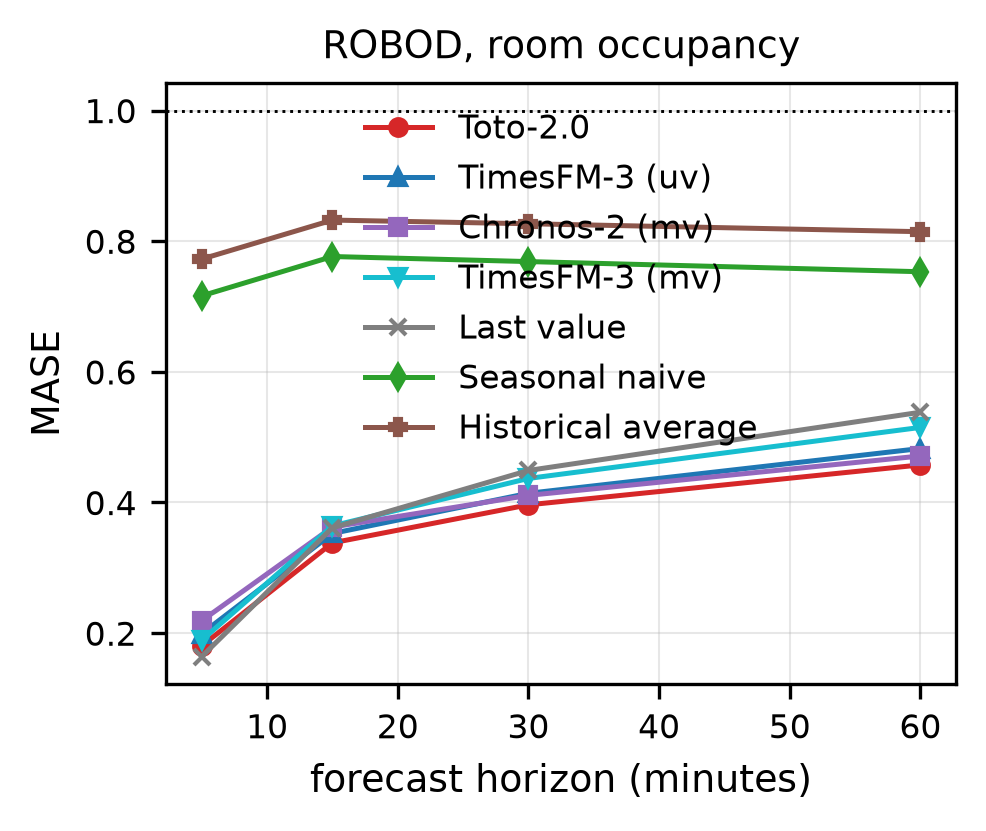
\includegraphics[width=\linewidth]{figures/skill_robod.png}
\caption{ROBOD, $S_m=0.44$.}
\end{subfigure}
\hfill
\begin{subfigure}{0.48\textwidth}
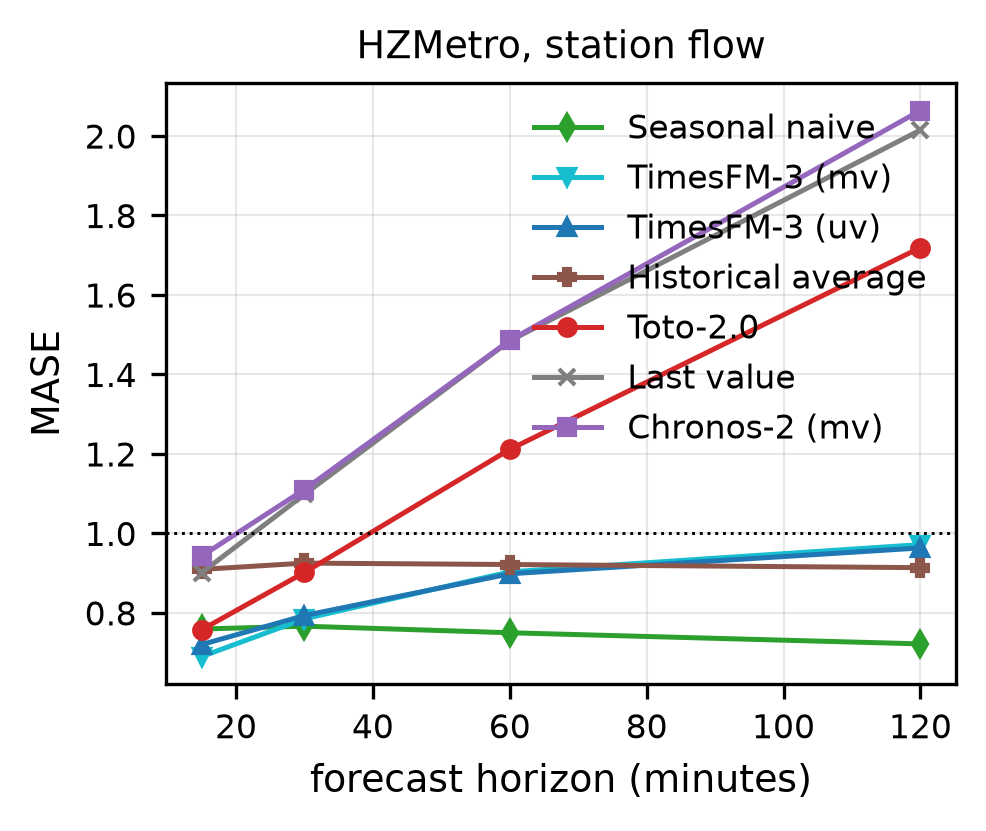
\includegraphics[width=\linewidth]{figures/skill_hzmetro.png}
\caption{HZMetro, $S_m=0.79$.}
\end{subfigure}
\caption{Accuracy against horizon on the two real datasets. The ordering reverses completely. On ROBOD the foundation models separate from the baselines as the horizon grows; on HZMetro the seasonal baseline is flat and unbeaten while the foundation models degrade. The dotted line at MASE \num{1} is the in-sample seasonal naive reference.}
\label{fig:skill}
\end{figure}

\subsection{H2: the predictability boundary}

Table~\ref{tab:hzmetro} reports HZMetro, and the result is the opposite of Table~\ref{tab:robod}. Seasonal naive attains \num{0.722} MASE at \SI{120}{\minute}, better than every foundation model at every horizon beyond \SI{15}{\minute}, and \emph{no} method significantly beats it anywhere under Diebold-Mariano with Holm control. The best zero-shot model trails it by \SI{33.5}{\percent} at \SI{120}{\minute}. Metro ridership is close to a deterministic function of time of day and day type, $S_m = 0.79$, and against a signal of that kind a forecaster that simply repeats yesterday is very hard to beat.

\begin{table}[htbp]
\centering
\caption{HZMetro, real station flow, \num{543}--\num{588} origins pooled over three seeds. No method significantly beats seasonal naive at any horizon; the daggers mark methods that significantly beat \emph{last value}, showing the tests do have power and that the null result against the seasonal baseline is not an artefact of a weak test.}
\label{tab:hzmetro}
\small
\begin{tabular}{lcccccccc}
\toprule
& \multicolumn{4}{c}{MASE} & \multicolumn{4}{c}{CRPS} \\
\cmidrule(lr){2-5}\cmidrule(lr){6-9}
Method & \SI{15}{\minute} & \SI{30}{\minute} & \SI{60}{\minute} & \SI{120}{\minute} & \SI{15}{\minute} & \SI{30}{\minute} & \SI{60}{\minute} & \SI{120}{\minute} \\
\midrule
\multicolumn{9}{l}{\emph{Zero-shot foundation models}}\\
TimesFM-3 (mv)          & \best{0.690}$^{\dagger}$ & 0.785$^{\dagger}$ & 0.903$^{\dagger}$ & 0.972$^{\dagger}$ & \best{21.63} & \best{24.76} & 28.77 & 31.69 \\
TimesFM-3 (uv)          & 0.720$^{\dagger}$ & 0.793$^{\dagger}$ & 0.898$^{\dagger}$ & 0.963$^{\dagger}$ & 22.51 & 25.02 & \best{28.58} & 31.34 \\
Toto-2.0                & 0.758$^{\dagger}$ & 0.902$^{\dagger}$ & 1.211$^{\dagger}$ & 1.719$^{\dagger}$ & 23.49 & 28.26 & 38.39 & 55.74 \\
Chronos-2 (mv)          & 0.943 & 1.110 & 1.486 & 2.064 & 29.46 & 34.61 & 46.84 & 66.50 \\
\midrule
\multicolumn{9}{l}{\emph{Baselines, no training}}\\
Seasonal naive          & 0.759 & \best{0.766}$^{\dagger}$ & \best{0.750}$^{\dagger}$ & \best{0.722}$^{\dagger}$ & 28.83 & 29.06 & 28.42 & \best{27.33} \\
Historical average      & 0.909 & 0.925 & 0.922$^{\dagger}$ & 0.914$^{\dagger}$ & 34.32 & 34.87 & 34.76 & 34.51 \\
Last value              & 0.901 & 1.098 & 1.484 & 2.015 & 30.27 & 37.62 & 52.14 & 72.19 \\
\bottomrule
\end{tabular}
\end{table}

Taken together with Table~\ref{tab:robod} this could look like an inconsistency, and it is the reason we consider the unconditional question ill-posed. Figure~\ref{fig:hypothesis} shows that it is not an inconsistency but an ordering. Across the three sites the zero-shot advantage falls monotonically as $S_m$ rises, from $+\SI{14.9}{\percent}$ at $S_m=0.44$, through $-\SI{4.0}{\percent}$ at $S_m=0.55$, to $-\SI{33.5}{\percent}$ at $S_m=0.79$, crossing zero at intermediate predictability. Every prediction Hypothesis~\ref{hyp:boundary} makes is borne out, including the sign change and the specific claim that no foundation model displaces the seasonal baseline at high $S_m$. Hypothesis~\ref{hyp:boundary} is supported.

\begin{figure}[htbp]
\centering
\begin{subfigure}{0.40\textwidth}
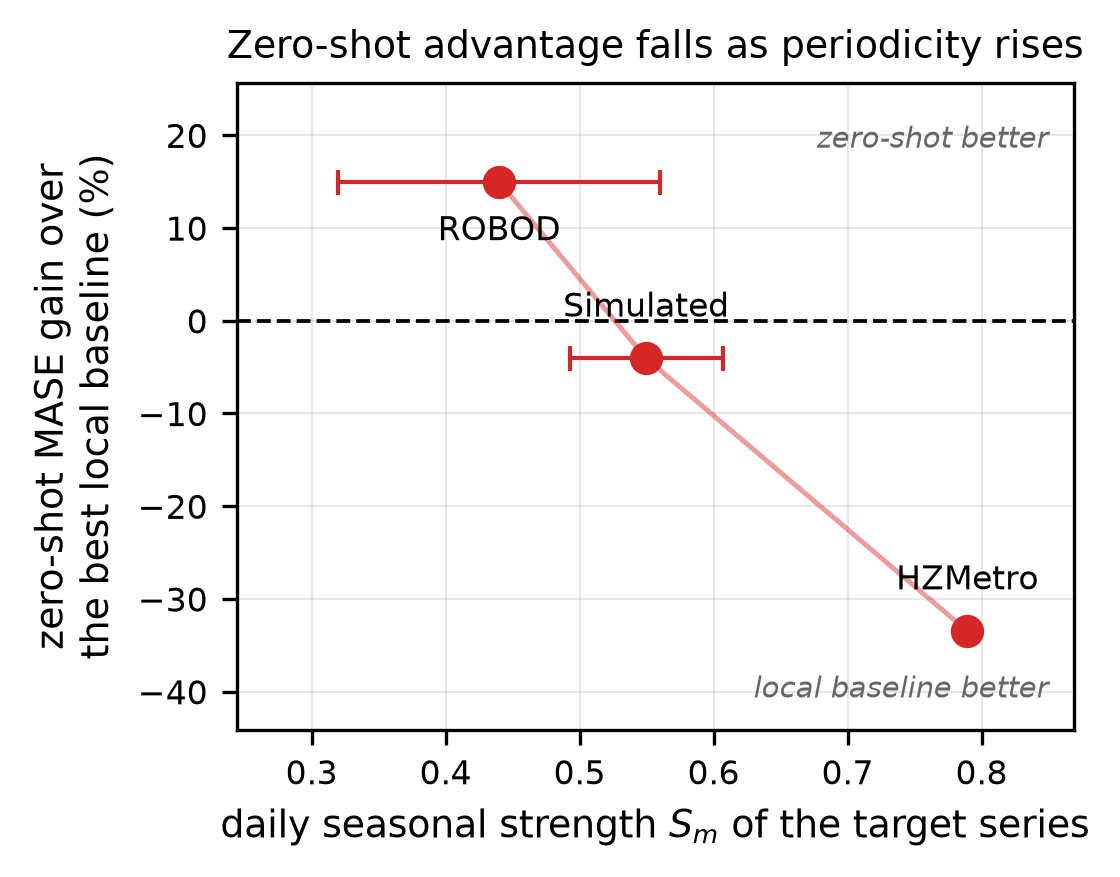
\includegraphics[width=\linewidth]{figures/hypothesis.png}
\caption{The predictability boundary.}
\label{fig:hypothesis}
\end{subfigure}
\hfill
\begin{subfigure}{0.56\textwidth}
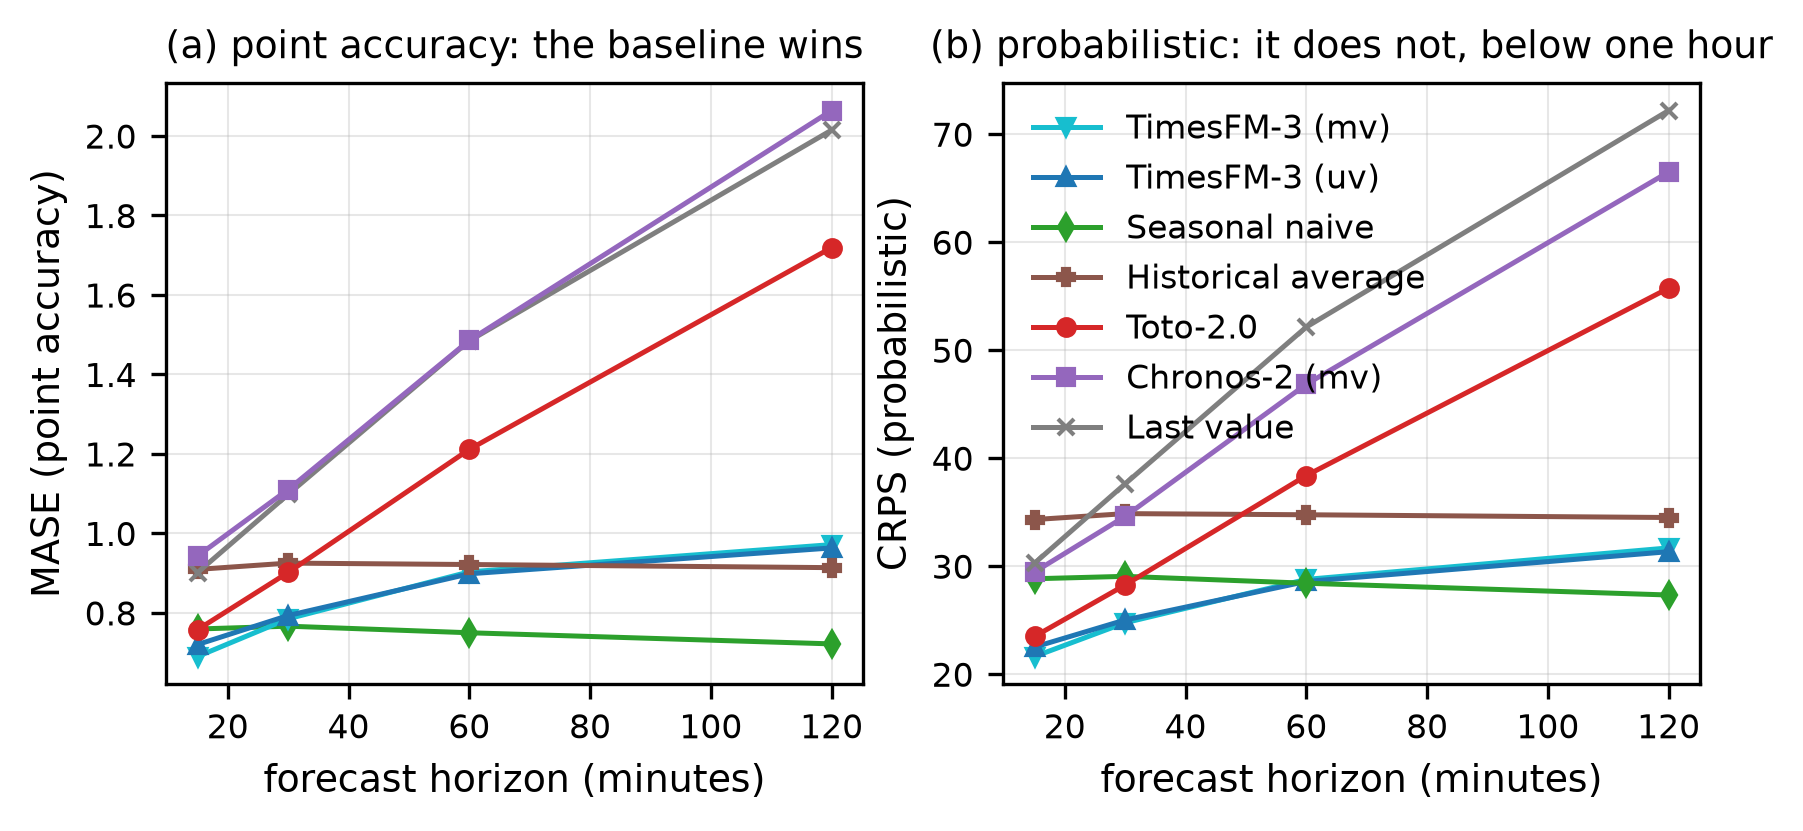
\includegraphics[width=\linewidth]{figures/point_vs_probabilistic.png}
\caption{HZMetro: point accuracy and probabilistic accuracy disagree.}
\label{fig:pointprob}
\end{subfigure}
\caption{Left: the zero-shot MASE advantage over the best local baseline, at the longest horizon of each experiment, against the daily seasonal strength of the target. Horizontal bars are the standard error of $S_m$ over series. Right: on the dataset where the seasonal baseline wins on MASE, it is beaten on CRPS at every horizon below one hour.}
\end{figure}

The practical consequence is that $S_m$ can be computed from a few weeks of counts before any model is procured, and it tells an operator which family to deploy. This is a considerably more useful statement than a leaderboard, and it is the reason we framed the study this way.

\subsection{H3: point accuracy and uncertainty come apart}

The conclusion of the previous section would be badly misleading if left there, because point accuracy is not what a protection system consumes. An alarm rule needs the probability that a threshold will be crossed, and that requires a calibrated distribution.

Table~\ref{tab:calibration} shows that the baselines winning on MASE are useless in this respect. Seasonal naive and historical average, as implemented with the deterministic quantiles they actually imply, emit intervals of zero width and therefore cover \SI{3.6}{\percent} to \SI{5.0}{\percent} of outcomes against a nominal \SI{80}{\percent}. The foundation models reach \SIrange{73.5}{85.8}{\percent} on HZMetro and \SIrange{88.2}{92.2}{\percent} on ROBOD. On CRPS, which scores the whole predictive distribution, TimesFM-3 leads the seasonal baseline at \SI{15}{\minute} (\num{21.6} against \num{28.8}, an improvement of \SI{25}{\percent}) and at \SI{30}{\minute}, and only loses beyond one hour, as Figure~\ref{fig:pointprob} shows. Hypothesis~\ref{hyp:uncertainty} is supported.

\begin{table}[htbp]
\centering
\caption{Empirical coverage of the nominal \SI{80}{\percent} interval, with mean interval width in persons. A method cannot support a probabilistic alarm rule without approximately correct coverage, and zero width means the forecast asserts certainty it does not possess.}
\label{tab:calibration}
\small
\begin{tabular}{lcccc}
\toprule
& \multicolumn{2}{c}{ROBOD (\SI{60}{\minute})} & \multicolumn{2}{c}{HZMetro (\SI{60}{\minute})} \\
\cmidrule(lr){2-3}\cmidrule(lr){4-5}
Method & coverage & width & coverage & width \\
\midrule
Toto-2.0            & 0.895 & 1.30 & 0.814 & 195.6 \\
Chronos-2 (mv)      & 0.907 & 1.57 & 0.853 & 233.3 \\
TimesFM-3 (uv)      & 0.884 & 1.35 & 0.758 & 141.4 \\
TimesFM-3 (mv)      & 0.882 & 1.31 & 0.778 & 145.7 \\
Last value          & 0.823 & 0.08 & 0.595 & 86.1 \\
Seasonal naive      & 0.707 & 0.00 & 0.042 & 0.0 \\
Historical average  & 0.639 & 0.00 & 0.034 & 0.0 \\
\bottomrule
\end{tabular}
\end{table}

This reframes the HZMetro result rather than reversing it. Where the signal is strongly periodic, a seasonal baseline is the better point predictor and should be used as such. But a heritage protection system does not act on point predictions, and the only methods here that supply a usable predictive distribution at any horizon are the foundation models. The honest recommendation that follows is a hybrid, and we state it in Section~\ref{sec:discussion}.

\subsection{H4: topology-blindness, measured and repaired}

Table~\ref{tab:recon} quantifies the motivating claim of the paper on the simulated museum, the only site reporting both sides of~\eqref{eq:conservation}. Raw foundation model forecasts violate the continuity equation by \num{1.05} persons per node per interval. In a house museum gallery whose typical occupancy is a handful of people this is not a rounding error: it means the forecast asserts that people appear in, or vanish from, rooms.

\begin{table}[htbp]
\centering
\caption{Reconciliation on the simulated museum, \num{600} paired forecast occasions (\num{300} origins $\times$ two forecasters), computed offline from stored quantile forecasts. Residual is the maximum absolute conservation violation and bound violation the total capacity and non-negativity violation, both in persons. $\Delta$MAE is the percentage change against the raw forecast, tested by a paired Wilcoxon signed-rank test over occasions. Solve time is the median in milliseconds. Only the proposed projection achieves all three of coherence, feasibility and improved accuracy.}
\label{tab:recon}
\small
\begin{tabular}{lrrrrlr}
\toprule
Reconciler & Residual & Bound viol. & MAE & $\Delta$MAE & $p$ & Solve \\
\midrule
None (raw forecast) & \num{1.049} & \num{0.006} & 0.3538 & reference & n/a & n/a \\
MinT (shrink)       & \num{3e-10} & \best{\num{1.738}} & 0.3556 & $+0.53$ & \num{2.2e-47} & \num{<0.1} \\
Uniform weight      & \num{7e-10} & \num{0.000} & 0.3548 & $+0.28$ & \num{1.6e-29} & 6.2 \\
\textbf{Proposed}   & \num{4e-9}  & \num{0.000} & \best{0.3511} & \best{$-0.76$} & \num{1.2e-2} & 10.2 \\
\bottomrule
\end{tabular}
\end{table}

All three reconcilers drive the conservation residual to solver tolerance, as Theorem~\ref{thm:unique} guarantees. The separation is in what they break on the way. MinT, which enforces the equalities by the linear map of Proposition~\ref{prop:mint} and has no representation of the box, introduces \num{1.738} persons of capacity and sign violation per origin. This is exactly the failure Proposition~\ref{prop:mint} predicts, and it is a consequential one: a reconciler that removes one class of physical impossibility by creating another has not delivered an admissible forecast. Both constrained projections leave the box exactly satisfied. Figure~\ref{fig:recon} shows the three criteria side by side; the proposed method is the only one that is not in the wrong on any of them. Hypothesis~\ref{hyp:coherence} is supported.

\begin{figure}[htbp]
\centering
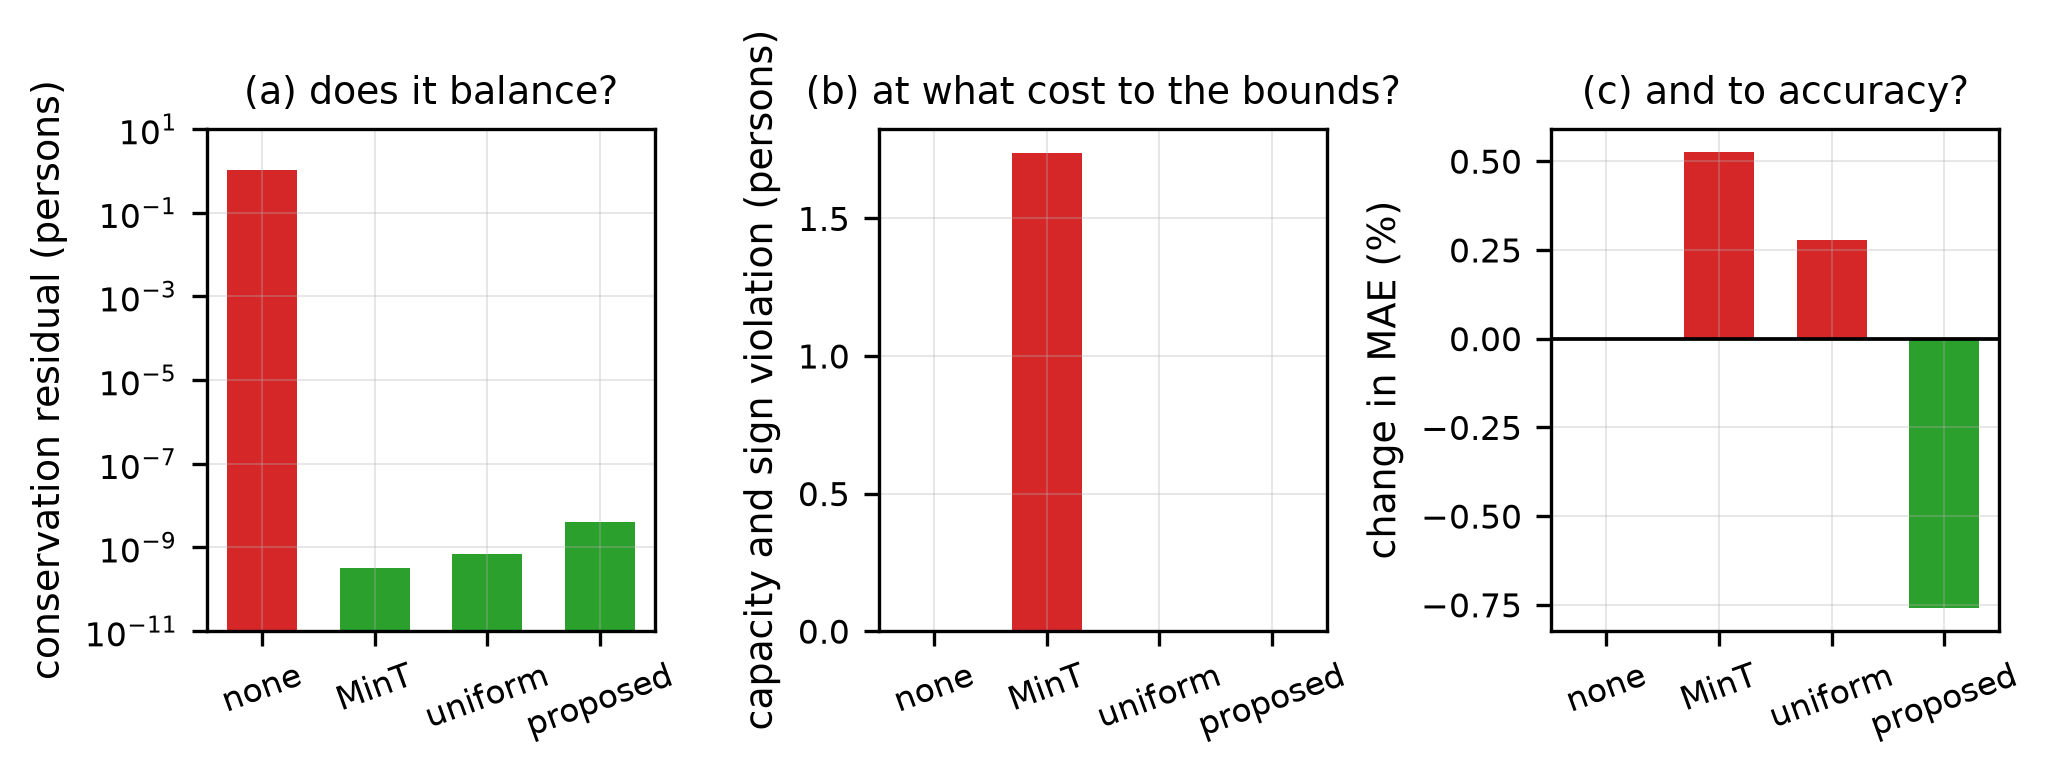
\includegraphics[width=0.95\textwidth]{figures/reconciliation.png}
\caption{Reconciliation must win on three criteria at once. (a) Every reconciler restores conservation. (b) Only MinT breaks the capacity and non-negativity constraints, as Proposition~\ref{prop:mint} predicts, because it has no representation of them. (c) Only the uncertainty-weighted projection improves point accuracy; uniform weighting enforces the same constraints and still degrades it. Green marks the desirable outcome.}
\label{fig:recon}
\end{figure}

\subsection{H5: the uncertainty weighting is what makes it pay}

The last two rows of Table~\ref{tab:recon} isolate the design decision this method rests on. The uniform and proposed arms solve the same quadratic program over the same admissible set, reach the same coherence and the same feasibility, and differ only in $\bOm$. Uniform weighting degrades MAE by \SI{0.28}{\percent} $(p=\num{1.6e-29})$: it fixes the physics and pays for it in accuracy. Weighting by the model's own quantile spread improves MAE by \SI{0.76}{\percent} $(p=\num{1.2e-2})$, and beats uniform weighting head to head by \SI{1.03}{\percent} on paired occasions $(p=\num{8.5e-34}$, $n=600)$. Hypothesis~\ref{hyp:weights} is supported.

The size of the point-accuracy gain is modest and we do not oversell it. Its importance is not the \SI{0.76}{\percent} but the sign, and the interpretation is precisely the one Corollary~\ref{cor:expected} anticipates. Theorem~\ref{thm:contraction} guarantees improvement in the $\bOm$-norm, not in MAE, so whether the guarantee survives the change of metric depends entirely on whether $\bOm$ points at the coordinates that were actually wrong. The uniform arm shows that when it does not, coherence is bought at a real cost in accuracy. The proposed arm shows that the quantile spread of a modern foundation model is informative enough about its own errors to convert that cost into a gain. To our knowledge this is the first direct evidence that a foundation model's predictive interval is useful as a reconciliation metric, and it is the practical reason the layer is worth adding rather than merely being defensible.

CRPS moves slightly the other way, from \num{0.2723} to \num{0.2729}. The shift strategy translates every quantile by the median correction and therefore holds interval widths fixed, so a shifted interval that is now correctly located may be marginally worse scored if the raw spread was already tuned to an incoherent median. We report this rather than selecting the strategy that hides it.

\subsection{Data efficiency and cost}

Figure~\ref{fig:efficiency} places the zero-shot model against a locally trained LightGBM given one to ninety days of site-specific data on the simulated museum. The trained model is already competitive at one day and saturates almost immediately, ending \SI{4.0}{\percent} ahead at \SI{60}{\minute}. We had pre-registered a crossover of at least two weeks and it did not occur: on a signal this periodic, a local model learns essentially all there is to learn within a day. That is a failed prediction on our part, and the same fact as the simulator's intermediate $S_m$ of \num{0.55}, so it is consistent with Hypothesis~\ref{hyp:boundary} while refuting the stronger data-efficiency claim we began with. The honest reading is that the cold start argument for foundation models is strong in the first hours of a deployment and on aperiodic signals, and weak on periodic ones after the first day.

\begin{figure}[htbp]
\centering
\begin{subfigure}{0.40\textwidth}
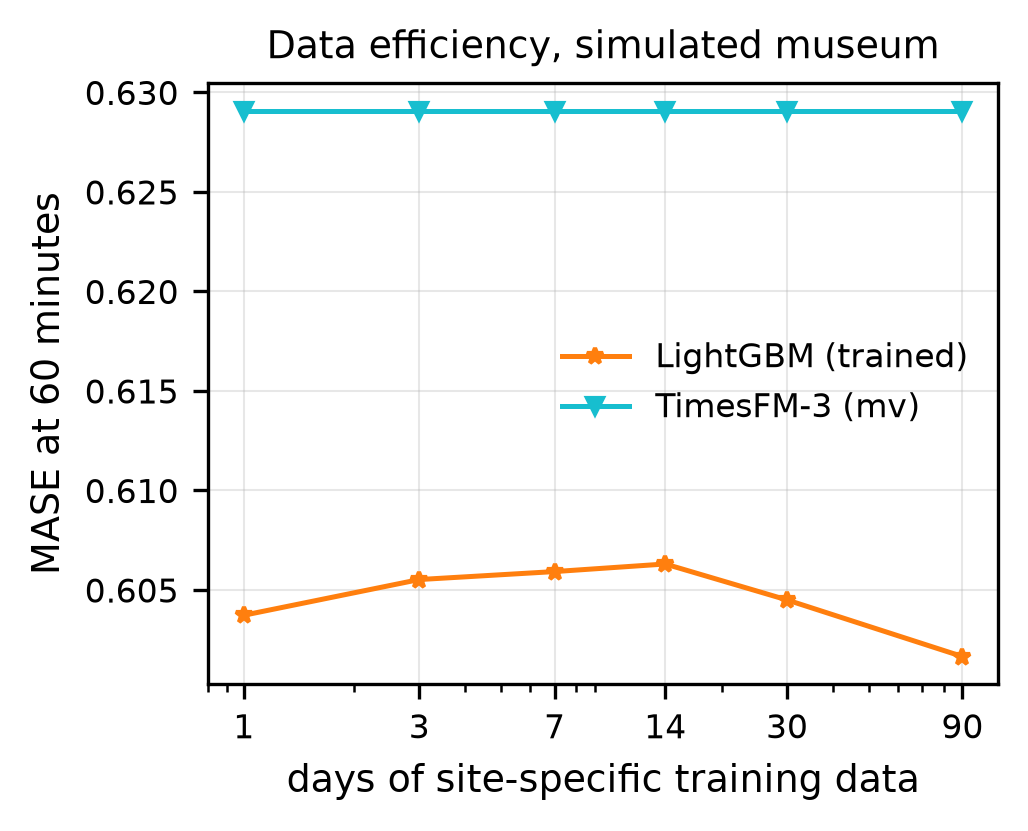
\includegraphics[width=\linewidth]{figures/data_efficiency.png}
\caption{Data efficiency, simulated museum.}
\label{fig:efficiency}
\end{subfigure}
\hfill
\begin{subfigure}{0.56\textwidth}
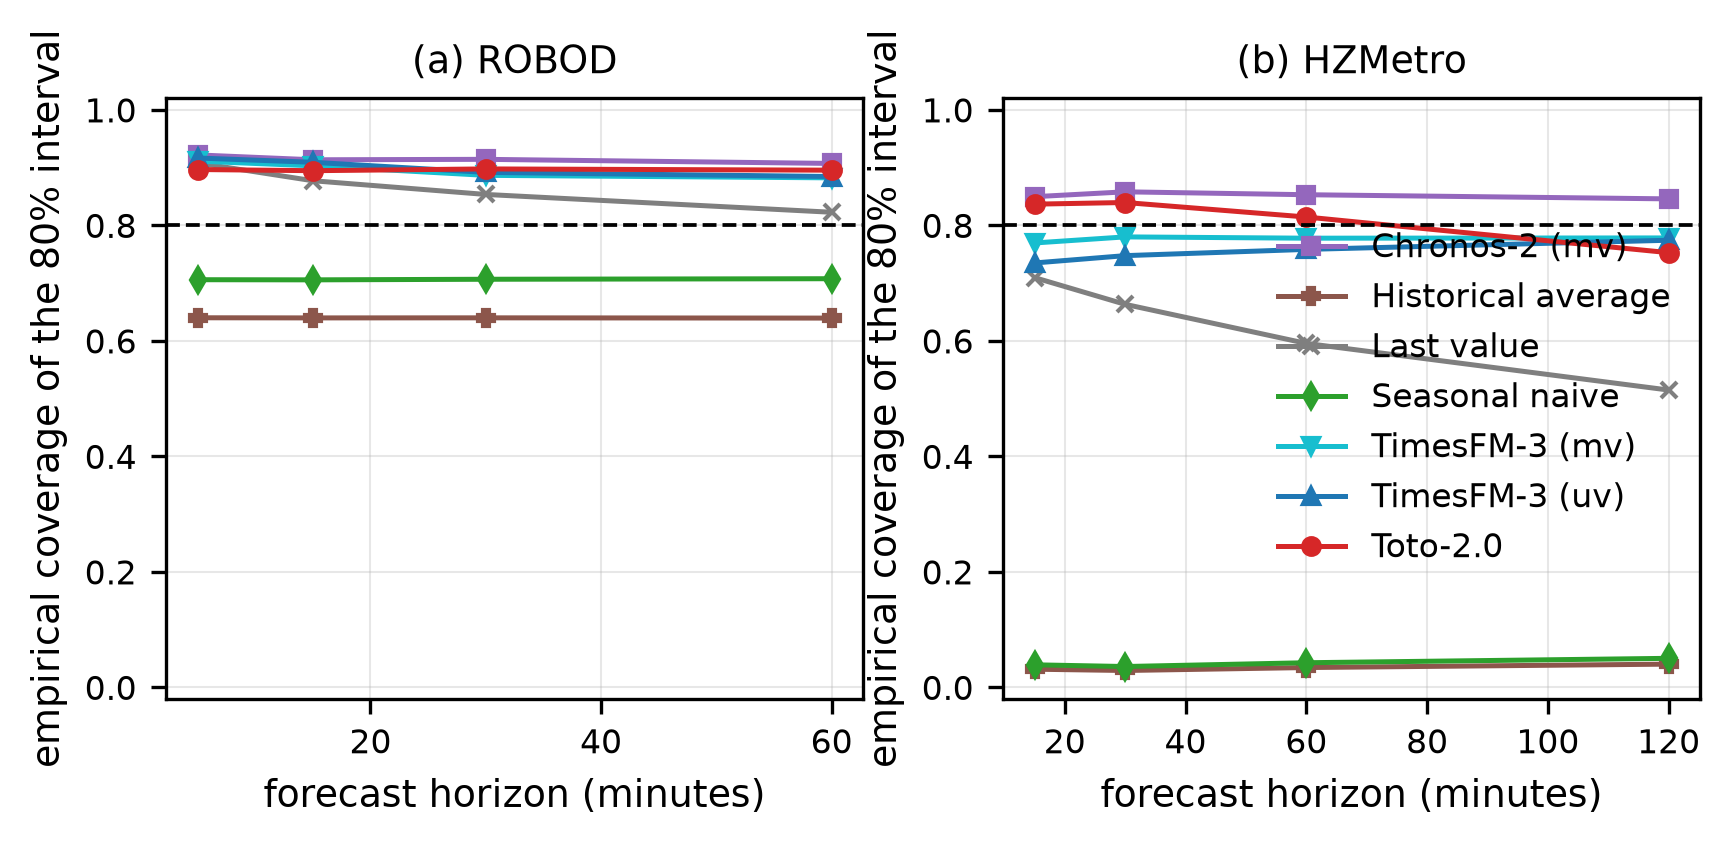
\includegraphics[width=\linewidth]{figures/calibration.png}
\caption{Calibration against horizon on both real sites.}
\label{fig:calibration}
\end{subfigure}
\caption{Left: a locally trained model saturates within a day on a strongly periodic simulated site, so the pre-registered two-week crossover does not occur. Right: empirical coverage of the nominal \SI{80}{\percent} interval, dashed. The seasonal baselines sit near zero on HZMetro because they emit zero-width intervals.}
\end{figure}

Cost is compatible with on-premise deployment, which matters because the privacy argument of Section~\ref{sec:related} depends on inference staying inside the building. On the \num{240}-series HZMetro panel the median per-origin latency on commodity hardware is \SI{152}{\milli\second} for Toto-2.0, \SI{207}{\milli\second} for TimesFM-3 multivariate and \SI{249}{\milli\second} for Chronos-2, against \SI{3}{\milli\second} for seasonal naive, with peak memory at or below \SI{1.4}{\mega\byte} beyond the model weights. The multivariate TimesFM-3 path is more than three times faster than its univariate path (\SI{676}{\milli\second}), since one forward pass replaces per-series calls. Reconciliation adds \SI{10.2}{\milli\second}. A forecast plus projection therefore completes in well under a second at the scale of any museum, against horizons of tens of minutes.

%=============================================================================
\section{Discussion}
\label{sec:discussion}
%=============================================================================

\paragraph{What to deploy.}
The results support a specific and slightly unfashionable recommendation. Compute $S_m$ on a few weeks of counts. Where it is low, as in the indoor occupancy setting this paper targets, deploy the foundation model, which wins on point accuracy, on distributional accuracy and on calibration at once. Where it is high, do not discard the seasonal baseline: use it for the conditional mean and the foundation model for the predictive distribution that the alarm rule consumes. That hybrid is not a compromise but a direct reading of Tables~\ref{tab:hzmetro} and~\ref{tab:calibration}, in which the two families win on different and separately necessary criteria. In both regimes apply the projection of Section~\ref{sec:method}, which costs \SI{10}{\milli\second}, guarantees physical admissibility, and does not cost accuracy when weighted by the model's own uncertainty.

\paragraph{Why multivariate mode is not uniformly better.}
TimesFM-3 in multivariate mode beats its univariate path on HZMetro at short horizons (\num{0.690} against \num{0.720} at \SI{15}{\minute}) and on ROBOD at \SI{5}{\minute}, but loses at longer horizons on both. We do not have a controlled ablation isolating the mechanism, since the covariate and multivariate experiments of our original design did not run, and we therefore make no claim about cross-series attention beyond reporting the measurements. We flag it as the most immediate open question, and note the caution of \citet{shao2022stid} that apparent gains from cross-series structure often have a simpler explanation.

\paragraph{Limitations.}
No real heritage museum pilot is included, and we make no deployment claim. The reconciliation result rests on the simulator, because neither public dataset measures occupancy and directional flow simultaneously, which is a gap in the available data rather than a modelling choice; a real site measuring both, such as dense indoor tracking, is the single most valuable addition to this evidence base and is our next step. The predictability hypothesis is confirmed on three datasets spanning $S_m \in [0.44,0.79]$, which establishes the ordering but does not locate the crossover precisely, and $S_m$ is a coarse summary that ignores whether the residual after the seasonal profile is itself predictable. The covariate, degradation and decision-utility experiments in our design remain unrun, so Hypotheses about known-future covariates and about operational lead time are neither supported nor refuted here; we state them as open rather than quietly dropping them. Finally, the ROBOD building is an office rather than a gallery, and although it is the closest public analogue in structure, the visitor population differs.

\paragraph{Ethics.}
The system counts and does not identify. Every claim rests on aggregate counts per space and per doorway, with no trajectories, no biometric data and no personal data leaving the building. This is a design constraint with a methodological consequence, since aggregate counting discards exactly the individual-level information trajectory methods rely on, which is why the problem is posed as forecasting on a graph. A deployment using device-based sensing would still warrant a data protection impact assessment under Article 35 of the GDPR \citep{gdpr}, and the same machinery would be open to misuse if paired with identifying sensors.

%=============================================================================
\section{Conclusion}
%=============================================================================

We asked whether a pre-trained time series foundation model can forecast visitor flow in a building it has never seen, and whether such a model can be made to respect the building's topology. On the first question the answer is conditional, and we identified the condition: the zero-shot advantage is a decreasing function of the daily seasonal strength of the target, confirmed without exception across $S_m$ from \num{0.44} to \num{0.79}, positive and significant at the low end and negative at the high end. Because $S_m$ is computable from history alone, this converts an empirical question into a decision rule available before any model is procured. Where the seasonal baseline wins on point accuracy it remains unusable for protection, since it covers \SI{4}{\percent} of outcomes against a nominal \SI{80}{\percent}, so the two families are complementary rather than competing.

On the second question the answer is affirmative and comes with proofs. The uncertainty-weighted constrained projection is unique, exactly coherent, and provably non-expansive towards any admissible truth, with MinT recovered as the special case that discards the inequality constraints and, as predicted and then measured, breaks them. Raw forecasts violate conservation by \num{1.05} persons per node per interval; the projection removes this in \SI{10.2}{\milli\second} while improving point accuracy, and the head-to-head comparison against uniform weighting shows the improvement comes specifically from using the model's own quantile spread as the metric. We release the simulated benchmark, the reconciliation layer and the harness, in which every reported number is traceable to a logged run.

%=============================================================================
\section*{Reproducibility statement}
%=============================================================================

All experiments are driven by versioned configuration files. Each run writes a manifest with the git commit, configuration hash, seed, package versions and hardware, alongside per-origin predictions and metrics. Every figure and table here is generated by one script from those artefacts, and it fails rather than emitting a placeholder when a run is missing. Public datasets are fetched by per-source scripts that record download date and checksum; the data itself is not redistributed.

\bibliographystyle{unsrtnat}
\bibliography{ref}

\end{document}
